\section{Leni izračun}
\label{sec:leni-izracun}

% Kaj je semantika, primerjava stroge in nestroge semantike
Semantika programskega jezika opisuje pravila in principe, ki določajo, kako se programi izvajajo. Semantiko za izračun izrazov v grobem delimo na strogo (angl. strict) in nestrogo (angl. non-strict). Večina programskih jezikov pri računanju izrazov uporablja strogo semantiko, ki določa, da se izrazi izračunajo \textit{takoj, ko so definirani}. Nasprotno, nestroga semantika določa, da se izrazi izračunajo šele, ko so dejansko potrebni za nadaljnjo obdelavo, oziroma se sploh ne izračunajo, če niso potrebni.

% Prevladovanje stroge semantike
Večina današnjih programskih jezikov temelji na strogi semantiki. Mednje spadajo tako imperativni jeziki, kot so npr. C, Rust, Python, kot tudi nekateri funkcijski programski jeziki, kot sta npr. Ocaml in Lisp. Jezikov, ki temeljijo na nestrogi semantiki je bistveno manj, med njimi npr. jeziki Haskell, Miranda in Clean.

% Primer
\begin{primer}[ht]
\centering
\begin{code-box}{haskell}{Haskell \cmark}
konjunkcija :: Bool -> Bool -> Bool
konjunkcija p q =
	case p of
		False -> False
		True -> q
\end{code-box}
\caption{Funkcija \var{konjunkcija} implementirana v lenem jeziku}
\label{pr:konjunkcija}
\end{primer}

Kot primer si oglejmo razliko pri izračunu izraza \texttt{konjunkcija False ((1 / 0) == 0)} (primer \ref{pr:konjunkcija}). Jeziki, ki temeljijo na strogi semantiki, ob klicu funkcije najprej izračunajo vrednosti argumentov. Ker pride pri izračunu drugega argumenta do napake, se izvajanje programa tukaj ustavi. Pri jezikih z nestrogo semantiko pa se ob klicu funkcije ne izračunajo vrednosti argumentov, temveč se računanje izvede šele takrat, ko je vrednost dejansko potrebovana. Ker je prvi argument pri klicu funkcije \texttt{False}, funkcija drugega argumenta ne izračuna in tako je rezultat klica vrednost \texttt{False}.

% Formalizacija stroge in nestroge semantike
Če semantika jezika dopušča izračun vrednosti izraza kljub temu, da vsi njegovi podizrazi niso izračunani, jo imenujemo nestroga semantika~\cite{peyton1987implementation}. Bolj formalno lahko uvedemo vrednost $\bot$, ki jo imenujemo tudi dno (angl. bottom) in predstavlja vrednosti izrazov, katerim ni mogoče izračunati normalne oblike (tj. izrazi, katerih vrednosti ne moremo izračunati oziroma izrazi, ki vrnejo napako). Če izraza \textit{expr} ne moremo izračunati, lahko tako zapišemo, da zanj velja $\textbf{eval}(expr) = \bot$. Za funkcijo enega argumenta pravimo, da je \textit{stroga}, če velja

\begin{equation*}
   f \: \bot = \bot
\end{equation*}

Za stroge funkcije enega argumenta torej velja, da če izračun argumenta pri klicu funkcije doseže dno (tj. vrednosti $\bot$), bo tudi rezultat funkcije napaka $\bot$. Če funkcija ni stroga, pravimo, da je nestroga.

% Kaj so neučakani in kaj so leni programski jeziki? 
Če programski jezik za izračun vrednosti izrazov uporablja strogo semantiko, pravimo, da je \emph{neučakan} (angl. eager). Vrednosti izrazov se pri neučakanem izračunu izračunajo takoj, ko se v programu pojavijo. Pri tem lahko izračun argumenta povzroči stranske učinke, katerih vrstni red in čas izvedbe sta ključna za nadaljnje delovanje programa, zato večina imperativnih jezikov uporablja neučakani izračun~\cite{peyton1987implementation}. Funkcijski programski jeziki, kot so npr. Scheme, ML ali OCaml, omogočajo uporabo stranskih učinkov in prav tako implementirajo neučakani izračun.

Če jezik implementira nestrogo semantiko, pravimo, da je \emph{len} (angl. lazy). Nestroga semantika torej matematično opiše aplikacijo funkcij v programskem jeziku, medtem ko je leni izračun \emph{način implementacije} nestroge semantike~\cite{peyton1987implementation}. Pri lenem izračunu se torej vrednost izraza ne izračuna takoj, ko je ta definiran, ampak šele, ko je njegova vrednost dejansko potrebna.

% Prednosti in slabosti
Ena glavnih pomanjkljivosti neučakanega izračuna je, da se pri klicu funkcije vedno izračunajo vse vrednosti argumentov, ne glede na to, ali bo vrednost posameznega argumenta v telesu funkcije sploh uporabljena. To pomeni, da lahko pride do nepotrebnega računanja, kar vpliva na učinkovitost programa. Prednost neučakanega izračuna pa je večja predvidljivost poteka programa~\cite{peyton1987implementation}, saj za razliko od lenega izračuna natanko vemo, kdaj se bo vrednost nekega izraza izračunala. Glavna prednost lenega izračuna je v tem, da se argumenti izračunajo \emph{največ enkrat}. Če argument v telesu funkcije ni uporabljen, se tudi nikoli ne izračuna. V primeru, da se uporabi, pa se njegova vrednost izračuna \textit{enkrat} in se nato memoizira za vse nadaljnje uporabe. Slabost lenega izračuna pa je težja implementacija in počasnejše izvajanje v primerjavi z jeziki, ki uporabljajo neučakan izračun~\cite{peyton1987implementation, sebesta2004concepts}.

% TODO: Reduction order - normal vs leftmost outmost

\subsubsection{Redukcija grafa}

% Razlika med imperativnimi in funkcijskimi jeziki - izvajanje
Zgodnejši programski jeziki so bili namenjeni neposrednemu upravljanju ra\-ču\-nal\-ni\-ka oziroma komuniciranju z vhodno izhodnimi napravami in so kot taki precej odražali delovanje računalniške arhitekture, na kateri so se izvajali~\cite{hudak1989conception}. Funkcijski programski jeziki omogočajo večji nivo abstrakcije, so bolj podobni matematični notaciji in posledično tudi bolj primerni za dokazovanje pravilnosti programov. Višji nivo abstrakcije pa pomeni, da jih je težje prevajati oziroma izvajati na današnji računalniški arhitekturi. Ena izmed ovir pri implementaciji lenega izračuna je učinkovito upravljanje z zakasnjenimi izrazi (angl. thunks) in zagotavljanje, da se ti izrazi izračunajo le, ko so resnično potrebni.

% Kako implementiramo leni izračun?
Leni izračun najpogosteje implementiramo s pomočjo redukcije gra\-fa~\cite{peyton1987implementation, hudak1989conception}. Pri tej metodi prevajalnik v pomnilniku najprej sestavi abstraktno sintaksno drevo programa, kjer vozlišča predstavljajo aplikacije funkcij oziroma operacije nad podatki, njihova podvozlišča pa odvisnosti med njimi. V procesu \textit{redukcije} se sintaksno drevo obdeluje z lokalnimi transformacijami, ki ga predelujejo, dokler ni dosežena končna oblika, tj. dokler ni izračunan rezultat programa. Pri tem se sintaksno drevo zaradi deljenja izrazov (angl. expression sharing) navadno spremeni v usmerjen graf.

Slika \ref{fig:redukcija-aplikacije-pred} prikazuje abstraktno sintaksno drevo izraza $(\lambda x \, . \, \textsc{not} \; x) \; \texttt{True}$. Aplikacija funkcij je predstavljena z vozliščem @, ki vsebuje dva podizraza: funkcijo, ki se bo izvedla, in njen argument. V tem primeru je funkcija anonimni lambda izraz $(\lambda x \, . \, \textsc{not} \; x)$, ki sprejme en argument. Pri redukciji se vse uporabe parametra $x$ zamenjajo z vrednostjo argumenta \texttt{True}. Slika \ref{fig:redukcija-aplikacije-po} prikazuje drevo po redukciji. Ker se je v funkciji argument $x$ pojavil le enkrat, je rezultat redukcije še vedno drevo.

\begin{figure*}[ht]
	\centering
	\begin{subfigure}[b]{0.45\textwidth}
		\centering
		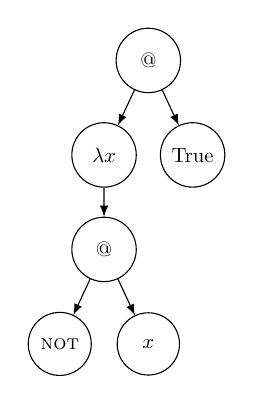
\begin{tikzpicture}[
			scale=0.75, transform shape,
			main/.style = {draw, circle},
			edge from parent/.style={draw,-latex},
			level distance=1.6cm,align=center,text width=0.75cm,
			]
			\node[main] (root) {@}
			child { node[main] {$\lambda x$}
				child { node[main] {@}
					child { node[main] {\textsc{not}} }
					child { node[main] {$x$} }
				}
			}
			child { node[main] {True} };
		\end{tikzpicture}
		\subcaption{Abstraktno sintaksno drevo \textit{pred} redukcijo}
		\label{fig:redukcija-aplikacije-pred}
	\end{subfigure}%
	\hfill
	\begin{subfigure}[b]{0.45\textwidth}
		\centering
		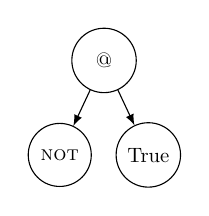
\begin{tikzpicture}[
			scale=0.75, transform shape,
			main/.style = {draw, circle},
			edge from parent/.style={draw,-latex},
			level distance=1.6cm,align=center,text width=0.75cm,
			]
			\node[main] (root) {@}
			child { node[main] {\textsc{not}} }
			child { node[main] {True} };
		\end{tikzpicture}
		\subcaption{Abstraktno sintaksno drevo \textit{po} redukciji}
		\label{fig:redukcija-aplikacije-po}
	\end{subfigure}
	\caption{Redukcija grafa izraza $(\lambda x \, . \, \textsc{not} \; x) \; \texttt{True}$}
	\label{fig:redukcija-aplikacije}
\end{figure*}

Slika \ref{fig:redukcija-dvojne-aplikacije} prikazuje en korak redukcije abstraktnega sintaksnega drevesa izraza $(\lambda x \, . \, \textsc{and} \; x \; x) \; (\textsc{not} \; \texttt{True})$. Po enem koraku redukcije sintaksnega telesa se \textit{vse uporabe} parametra $x$ zamenjajo z njegovo vrednostjo. Ker je takih pojavitev več, pa rezultat ni več drevo, temveč acikličen usmerjen graf. V pomnilniku tak izraz predstavimo z dvema kazalcema na isti objekt. Ko se objekt prvič izračuna, se vrednost objekta v pomnilniku posodobi z izračunano vrednostjo. Ob vseh nadaljnjih uporabah argumenta tako ne bo potrebno še enkrat računati njegove vrednosti, s čimer dosežemo, da bo vsak argument izračunan največ enkrat. 

\begin{figure*}[ht]
	\centering
	\begin{subfigure}[b]{0.45\textwidth}
		\centering
		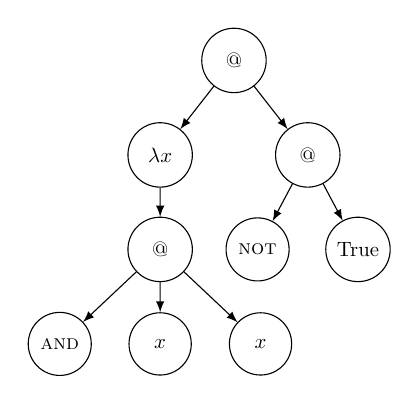
\begin{tikzpicture}[
			scale=0.75, transform shape,
			main/.style = {draw, circle},
			edge from parent/.style={draw,-latex},
			level distance=1.6cm,align=center,text width=0.75cm,
			level 1/.style={sibling distance=2.5cm},
			level 2/.style={sibling distance=1.7cm},
			]
			\node[main] (root) {@}
			child { node[main] {$\lambda x$}
				child { node[main] {@}
					child { node[main] {\textsc{and}} }
					child { node[main] {$x$} }
					child { node[main] {$x$} }
				}
			}
			child { node[main] {@}
				child { node[main] {\textsc{not}} }
				child { node[main] {True} }
			};
		\end{tikzpicture}
	\end{subfigure}%
	\hfill
	\begin{subfigure}[b]{0.45\textwidth}
		\centering
		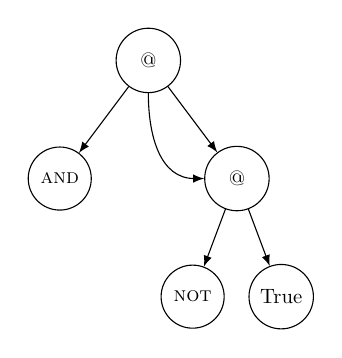
\begin{tikzpicture}[
			scale=0.75, transform shape,
			main/.style = {draw, circle},
			edge from parent/.style={draw,-latex},
			level distance=2cm,align=center,text width=0.75cm,
			]
			\node[main] (root) {@}
			child { node[main] {\textsc{and}} }
			child { edge from parent[draw=none] }
			child { node[main] (argument) {@}
				child { node[main] {\textsc{not}} }
				child { node[main] {True} }
			};
			\draw[-latex] (root) to[out=-90, in=180, looseness=1.1] (argument);
		\end{tikzpicture}
	\end{subfigure}
	\caption{Redukcija grafa izraza $(\lambda x \, . \, \textsc{and} \; x \; x) \; (\textsc{not} \; \texttt{True})$}
	\label{fig:redukcija-dvojne-aplikacije}
\end{figure*}

Slika \ref{fig:funkcija-y} prikazuje dve možni implementaciji ciklične funkcije $Y \; f = f \; (Y \; f)$. Za razliko od primerov na slikah \ref{fig:redukcija-aplikacije} in \ref{fig:redukcija-dvojne-aplikacije}, pri katerih je bilo reducirano sintaktično drevo še vedno usmerjen acikličen graf, pa temu pri funkciji $Y$ ni več tako. Funkcija $Y$ je namreč rekurzivna, kar pomeni, da se sama pojavi kot vrednost svojega argumenta. Na sliki \ref{fig:funkcija-y-kot-prosta-spremenljivka} je funkcija $Y$ implementirana s pomočjo acikličnega grafa, a v svojem telesu vseeno dostopa do proste spremenljivke $Y$, zaradi česar obstaja v pomnilniku cikel. Na sliki \ref{fig:funkcija-y-kot-cikel} je funkcija implementirana neposredno s pomnilniškim ciklom, kjer je vrednost argumenta kar vozlišče samo.

\begin{figure*}[ht]
	\centering
	\begin{subfigure}[b]{0.45\textwidth}
		\centering
		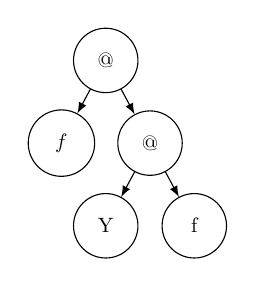
\begin{tikzpicture}[
			scale=0.75, transform shape,
			main/.style = {draw, circle},
			edge from parent/.style={draw,-latex},
			level distance=1.4cm,align=center,text width=0.75cm,
			]
			\node[main] (root) {@}
			child { node[main] {$f$} }
			child { node[main] {@}
				child { node[main] {Y} }
				child { node[main] {f} }
			};
		\end{tikzpicture}
		\subcaption{Funkcija $Y$, implementirana z uporabo proste spremenljivke}
		\label{fig:funkcija-y-kot-prosta-spremenljivka}
	\end{subfigure}%
	\hfill
	\begin{subfigure}[b]{0.45\textwidth}
		\centering
		\begin{tikzpicture}[
			scale=0.75, transform shape,
			main/.style = {draw, circle},
			edge from parent/.style={draw,-latex},
			level distance=1.4cm,align=center,text width=0.75cm,
			]
			\node[main] (root) {@}
			child { node[main] {$f$} }
			child { node (right) {} edge from parent[draw=none] };
			\coordinate [above=0.6cm of root] (above-root);
			\coordinate [right=0.4cm of right] (right-of-right);
			\coordinate (intermediate) at (right-of-right |- above-root);
			\draw[-latex] (root) -- (right.center) -- (right-of-right) -- (intermediate) -- (above-root) -- (root.north);
		\end{tikzpicture}
		\subcaption{Funkcija $Y$, implementirana kot cikličen usmerjen graf}
		\label{fig:funkcija-y-kot-cikel}
	\end{subfigure}
	\caption{Graf funkcije $Y \; f = f \; (Y \; f)$}
	\label{fig:funkcija-y}
\end{figure*}

\subsubsection{Zapis grafa v pomnilniku}

Leni izračun najpogosteje implementiramo s pomočjo zakasnjenih izrazov oziroma zakasnitev (angl. thunks). Te so v pomnilniku predstavljene kot ovojnice, tj. strukture s kazalcem na kodo, ki izračuna njihovo vrednost, in polji, ki vsebujejo vezane in proste spremenljivke. Ob izračunu zakasnitve (angl. forcing a thunk) se najprej izračuna njena vrednost, nato pa se izračunana vrednost shrani v strukturo v pomnilniku, da je ob naslednji uporabi ni potrebno ponovno računati. Pravimo, da se vrednost v pomnilniku \emph{posodobi}. Tako v programskem jeziku zagotovimo nestrogo semantiko, pri kateri se vsak izraz izračuna \textit{največ enkrat}. Če se argument ne pojavi nikjer v telesu funkcije, se zakasnitve nikoli ne računa, če pa se v telesu pojavi večkrat, se vrednost izračuna enkrat, za vsak nadaljnji izračun argumenta pa se preprosto vrne vrednost, shranjeno v pomnilniku.

Slika \ref{fig:shema-vozlisca-pomnilnik} prikazuje eno izmed možnih predstavitev vozlišča grafa. Sestavljena je iz oznake vozlišča in polj z vsebino oziroma argumenti $a_1, \dots, a_n$.  Oznaka je vrednost, ki predstavlja vrsto vozlišča: aplikacija funkcije, primitivna operacija, celoštevilska vrednost, preusmeritev, ipd. V poglavju \ref{sec:stg-definicija} bomo videli, da sta si struktura \ref{fig:shema-vozlisca-pomnilnik} in pomnilniški zapis objektov v jeziku STG precej podobna.

\begin{figure*}[ht]
	\centering
	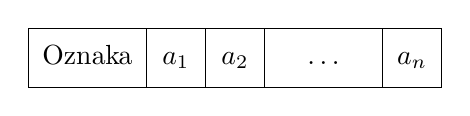
\begin{tikzpicture}[
		% Popravi vertikalno pozicioniranje teksta
		% https://tex.stackexchange.com/a/133237/324113
		verticalalign/.append style={font=\vphantom{Ag}},
		scale=0.75,
		]
		\draw[verticalalign] (0,0) rectangle ++(2,1) node[midway] {Oznaka};
		\draw[verticalalign] (2,0) rectangle ++(1,1) node[midway] {$a_1$};
		\draw[verticalalign] (3,0) rectangle ++(1,1) node[midway] {$a_2$};
		\draw[verticalalign] (4,0) rectangle ++(2,1) node[midway] {$\dots$};
		\draw[verticalalign] (6,0) rectangle ++(1,1) node[midway] {$a_n$};
	\end{tikzpicture}
	\caption{Pomnilniška predstavitev vozlišča grafa}
	\label{fig:shema-vozlisca-pomnilnik}
\end{figure*}

Slika \ref{fig:leni-izracun-pomnilnik-izraz} prikazuje predstavitev izraza $\textsc{and} \; (\textsc{not} \; \texttt{True}) \; (\textsc{not} \; \texttt{True})$ v pomnilniku. Celoten izraz je sestavljen iz dveh ovojnic, ki predstavljata dve aplikaciji. Spodnja ovojnica predstavlja izraz $\textsc{not} \; \texttt{True}$ in je sestavljena kot aplikacija funkcije \textsc{not} na argument z vrednostjo \texttt{0x0001}, tj. vrednost \texttt{True}. Zgornja ovojnica predstavlja aplikacijo funkcije \textsc{and} na dva argumenta, ki sta predstavljena kot kazalca na drugo ovojnico. Ko se izraz $\textsc{not} \; \texttt{True}$ prvič izračuna, se ovojnica v pomnilniku posodobi z iz\-ra\-ču\-na\-no vrednostjo. Pri tem se navadno v pomnilniku ustvari nova struktura, ovojnico pa se prepiše s preusmeritvijo na novonastalo strukturo. Tako ob vseh nadaljnjih dostopih vrednosti ovojnice ni potrebno ponovno računati.

\begin{figure*}[ht]
	\centering
	\begin{tikzpicture}[scale=0.8]
		\draw (0,0) rectangle ++(1,1) node[midway] {\textbf{@}};
		\draw (1,0) rectangle ++(2,1) node[midway] (and) {};
		\draw (3,0) rectangle ++(2,1) node[midway] (and-arg1) {};
		\draw (5,0) rectangle ++(2,1) node[midway] (and-arg2) {};
		
		\draw (0,-2) rectangle ++(1,1) node[midway] (app-not) {\textbf{@}};
		\draw (1,-2) rectangle ++(2,1) node[midway] (not) {};
		\draw (3,-2) rectangle ++(2,1) node[midway] {\texttt{0x0001}};
		
		\node (above-and) at (2,2) {\textsc{and}};
		\node (below-not) at (2,-3) {\textsc{not}};
		
		\draw[Circle-] (4,0.5) -- ++(0,-1);
		\draw[Circle-Latex] (6,0.5) -- ++(0,-1) -- ++(-7,0) -- ++(0,-1) -- ++(1,0);
		
		\draw[Circle-Latex] (2,0.5) -- ++(0,1);
		\draw[Circle-Latex] (2,-1.5) -- ++(0,-1);
		% \draw[-latex] (and) -- (above-and);
	\end{tikzpicture}
	\caption{Predstavitev izraza $\textsc{and} \; (\textsc{not} \; \texttt{True}) \; (\textsc{not} \; \texttt{True})$ v pomnilniku}
	\label{fig:leni-izracun-pomnilnik-izraz}
\end{figure*}

Ena izmed slabosti jezikov z lenim izračunom je, da je za razliko od neučakanih imperativnih jezikov zelo težko predvideti, koliko prostora bo program porabil. Ker so v takih jezikih funkcije navadno obravnavane kot primitivi, kar pomeni, da lahko nastopajo kot vrednost argumenta ali rezultata, je lahko njihovo izvajanje zamaknjeno v čas po koncu izvajanja funkcije, ki je ustvarila vrednost argumenta ali rezultata. Zato klicnih zapisov takih funkcij ni mogoče hraniti na skladu, temveč jih moramo hraniti na kopici~\cite{jones2023garbage}. Pri izvajanju se tako na kopici nenehno ustvarjajo in brišejo nove ovojnice, ki imajo navadno zelo kratko življenjsko dobo, zato je nujna učinkovita implementacija dodeljevanja in sproščanja pomnilnika. Haskell za to uporablja \textit{generacijski} avtomatični čistilec pomnilnika~\cite{sansom1993generational, GHC}. Danes vsi večji funkcijski programski jeziki, ki omogočajo leni izračun, uporabljajo avtomatični čistilec pomnilnika~\cite{turner1985miranda, czaplicki2012elm, brus1987clean, syme2017the, sperber2009revised6}.